\documentclass[12pt,a4paper]{article}

% ---------- Packages ----------
\usepackage[a4paper,margin=2.2cm]{geometry}
\usepackage{graphicx}
\usepackage{xcolor}
\usepackage{booktabs}
\usepackage{listings}
\usepackage{tikz}
\usetikzlibrary{shapes.geometric, arrows.meta, positioning}
\usepackage{hyperref}
\usepackage{titlesec}
\usepackage{fancyhdr}
\usepackage{enumitem}
\usepackage{caption}
\usepackage{tabularx}
\usepackage{float}

% ---------- Colors ----------
\definecolor{accent}{HTML}{B3304A}
\definecolor{codebg}{HTML}{F4F4F8}
\definecolor{codekw}{HTML}{0B5FA5}
\definecolor{codestr}{HTML}{16794B}
\definecolor{codecmt}{HTML}{6B7280}

% ---------- Section styling ----------
\titleformat{\section}
  {\large\bfseries\color{accent}}{\thesection}{0.6em}{}
\titleformat{\subsection}
  {\bfseries\color{black}}{\thesubsection}{0.6em}{}
\titlespacing{\section}{0pt}{14pt}{8pt}
\titlespacing{\subsection}{0pt}{10pt}{6pt}

% ---------- Header/Footer ----------
\pagestyle{fancy}
\fancyhf{}
\renewcommand{\headrulewidth}{0.4pt}
\fancyhead[L]{\small Smart Cane Environmental Awareness System}
\fancyhead[R]{\small Final Report}
\fancyfoot[C]{\thepage}

% ---------- Code listing style ----------
\lstdefinestyle{pystyle}{
  language=Python,
  backgroundcolor=\color{codebg},
  basicstyle=\ttfamily\small,
  keywordstyle=\color{codekw}\bfseries,
  stringstyle=\color{codestr},
  commentstyle=\color{codecmt}\itshape,
  numbers=left,
  numberstyle=\tiny\color{gray},
  frame=single,
  rulecolor=\color{gray!40},
  breaklines=true,
  showstringspaces=false,
  tabsize=4,
  xleftmargin=1.5em,
  framexleftmargin=1.2em,
}
\lstset{style=pystyle}

\hypersetup{
  colorlinks=true,
  linkcolor=accent,
  urlcolor=accent,
  citecolor=accent,
}

\title{}
\author{}
\date{}

\begin{document}

% ===================================================================
% TITLE PAGE
% ===================================================================
\begin{titlepage}
\centering
\vspace*{2cm}

{\Huge\bfseries AI Smart Navigation Assistant for\\[0.3cm] Visually Impaired People\\[0.3cm] Using Raspberry Pi}

\vspace{0.6cm}
{\Large\color{accent}\textit{Smart Cane Environmental Awareness System}}

\vspace{1.5cm}
{\large Final Project Report}

\vspace{2cm}
{\large\bfseries Igor Xavier \quad $\cdot$ \quad Fang Jialuo}

\vspace{0.5cm}
{\normalsize IoT Term Project}

\vfill

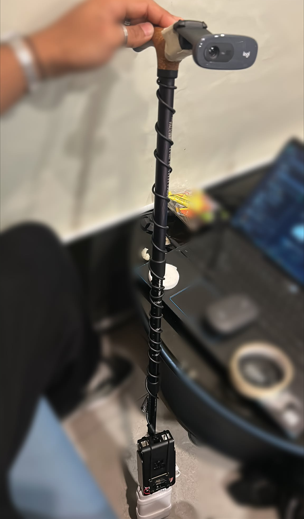
\includegraphics[height=6.5cm,keepaspectratio]{../photos/hardwarePhoto2.png}

\vspace{1cm}
{\normalsize Repository: \url{https://github.com/w1ggor/smart-nav-cane}}

\vspace{0.5cm}
{\normalsize \today}

\end{titlepage}

% ===================================================================
% ABSTRACT
% ===================================================================
\section*{Abstract}

This report presents the design and implementation of a Smart Cane Environmental Awareness System: an offline, edge-AI assistive device for visually impaired users built entirely on a Raspberry Pi 4. The system combines a Time-of-Flight (ToF) depth camera, a USB webcam, and Bluetooth audio to provide three capabilities: (1) real-time obstacle detection and classification, (2) visual place recognition for trained indoor locations, and (3) voice-driven guided navigation with turn-by-turn audio instructions. The project deliberately combines classical computer vision (ORB feature matching) with deep learning (YOLOv8-nano for object classification, and a neural acoustic model inside Vosk for offline speech recognition), choosing each technique where it is most appropriate for a resource-constrained embedded platform. The system runs with no internet connection and no cloud dependency. We describe the architecture, hardware, software implementation, the engineering challenges encountered while integrating real hardware, and the current results, before outlining future work toward full indoor navigation.

\vspace{0.5cm}
\noindent\textbf{Keywords:} Raspberry Pi, assistive technology, edge AI, deep learning, object detection, speech recognition, computer vision, offline navigation.

\vspace{1cm}
\tableofcontents

\newpage

% ===================================================================
\section{Project Idea}
% ===================================================================

\subsection{Motivation}
Visually impaired individuals face daily challenges navigating indoor environments safely and independently, particularly in unfamiliar or changing spaces. Commercial assistive devices that solve this problem comprehensively (e.g. devices using full SLAM-based mapping) are expensive and depend on specialized hardware such as inertial measurement units (IMUs) or LiDAR. Our goal was to build a low-cost, fully offline assistive device using commodity hardware that a student project can realistically build and demonstrate within an academic term.

\subsection{Core Concept}
The system is shaped like, and worn or carried like, a cane. It listens for a spoken destination, then guides the user there while continuously watching for obstacles and announcing them aloud through Bluetooth headphones. Three questions drive the entire design:

\begin{enumerate}[leftmargin=1.4cm]
  \item \textbf{What is in front of me?} — Obstacle detection (depth) and obstacle classification (deep learning).
  \item \textbf{Where am I?} — Visual place recognition against previously trained locations.
  \item \textbf{How do I get to my destination?} — Voice-driven guided navigation with turn-by-turn audio.
\end{enumerate}

\subsection{Scope Decision}
The original project vision considered full indoor mapping using Visual SLAM (e.g. ORB-SLAM3) to build a 3D map and plan routes autonomously. After evaluating the available hardware — no IMU, no wheel odometry, a single Raspberry Pi 4 CPU — we determined that full SLAM was not achievable within the project timeline with acceptable reliability. We therefore redesigned the system around two achievable, complementary modes described in Section~\ref{sec:design}, while preserving the original vision explicitly as future work (Section~\ref{sec:future}).

\subsection{Related Approaches}
Commercial and research assistive navigation devices typically fall into two categories. \textbf{Sensor-fusion SLAM systems} (e.g. wearable LiDAR + IMU rigs) build a persistent 3D map and can route to unseen destinations, but require expensive sensors and significant onboard compute, putting them out of reach for a low-cost student prototype. \textbf{Simple sensory substitution devices} (e.g. ultrasonic canes that simply beep when close to an obstacle) are cheap and reliable but provide no semantic information — the user is warned \emph{that} something is near, not \emph{what} it is or \emph{where they are}. This project deliberately sits between the two: it adds semantic understanding (object classification, place recognition, voice interaction) on top of low-cost depth sensing, without requiring the full sensor suite SLAM depends on.

\subsection{Classical Computer Vision vs.\ Deep Learning in This Project}
A central design decision was choosing, for each recognition task, whether classical computer vision or a learned model was more appropriate given the constraints of a single-board computer with no GPU. Table~\ref{tab:cv-vs-dl} summarizes this reasoning, which is revisited in more depth in Section~\ref{sec:ai}.

\begin{table}[H]
\centering
\begin{tabularx}{\textwidth}{l X X X}
\toprule
\textbf{Technique} & \textbf{Type} & \textbf{Training data needed} & \textbf{Used for} \\
\midrule
ORB + BFMatcher & Classical CV (hand-engineered features) & A 2-minute capture session per location/landmark, no labeling & Place and landmark recognition \\
YOLOv8-nano & Deep learning (CNN, pretrained) & None (uses public COCO weights) & Classifying generic obstacles (chair, person, etc.) \\
Vosk acoustic model & Deep learning (DNN-HMM, pretrained) & None (uses public English model) & Offline speech-to-text for destination input \\
\bottomrule
\end{tabularx}
\caption{Recognition techniques used in the project, contrasted by type and data requirements.}
\label{tab:cv-vs-dl}
\end{table}

% ===================================================================
\section{System Design \& Methodology}
\label{sec:design}
% ===================================================================

\subsection{Architecture Overview}

\begin{figure}[H]
\centering
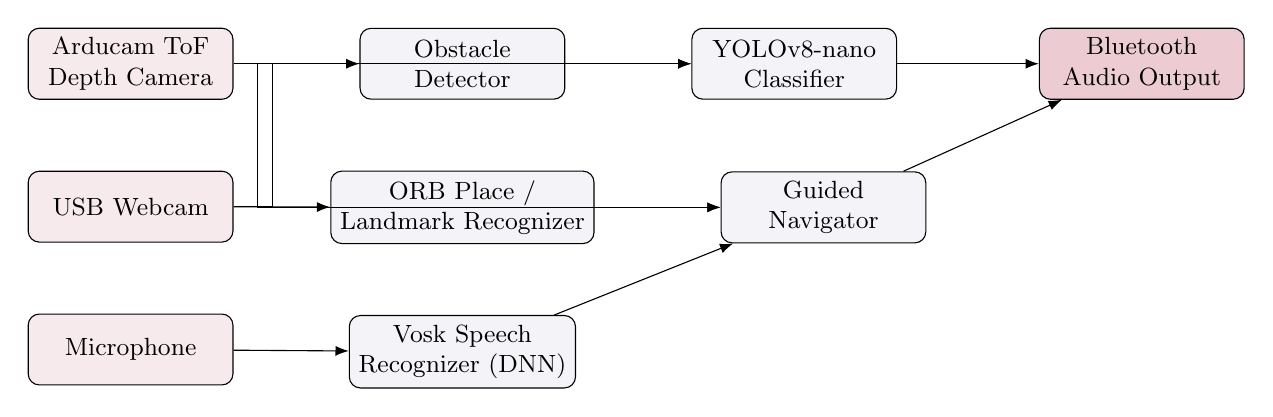
\begin{tikzpicture}[
  box/.style={rectangle, draw, rounded corners, minimum height=0.9cm, minimum width=2.6cm, align=center, font=\small},
  sensor/.style={box, fill=accent!10},
  proc/.style={box, fill=codebg},
  node distance=0.9cm and 1.0cm
]
\node[sensor] (tof) {Arducam ToF\\Depth Camera};
\node[sensor, below=of tof] (cam) {USB Webcam};
\node[sensor, below=of cam] (mic) {Microphone};

\node[proc, right=1.6cm of tof] (obs) {Obstacle\\Detector};
\node[proc, below=of obs] (orb) {ORB Place /\\Landmark Recognizer};
\node[proc, below=of orb] (stt) {Vosk Speech\\Recognizer (DNN)};

\node[proc, right=1.6cm of obs] (yolo) {YOLOv8-nano\\Classifier};
\node[proc, right=1.6cm of orb] (nav) {Guided\\Navigator};

\node[sensor, right=1.8cm of yolo, fill=accent!25] (audio) {Bluetooth\\Audio Output};

\draw[-Latex] (tof) -- (obs);
\draw[-Latex] (cam) -- (orb);
\draw[-Latex] (mic) -- (stt);
\draw[-Latex] (obs) -- (yolo);
\draw[-Latex] (cam.east) -- ++(0.5,0) |- (yolo.west);
\draw[-Latex] (orb) -- (nav);
\draw[-Latex] (tof.east) -- ++(0.3,0) |- (nav.west);
\draw[-Latex] (stt) -- (nav);
\draw[-Latex] (yolo) -- (audio);
\draw[-Latex] (nav) -- (audio);
\end{tikzpicture}
\caption{High-level data flow. Sensors (left) feed both classical CV and DL processing stages (center), which converge on the audio output (right).}
\label{fig:architecture}
\end{figure}

The system runs two distinct operating modes built from the same underlying modules:

\begin{itemize}[leftmargin=1.4cm]
  \item \textbf{Awareness mode} — a continuous 2~Hz loop that detects obstacles and passively announces recognized locations, with no destination.
  \item \textbf{Guided navigation mode} — the user speaks a destination; the system gives turn-by-turn audio guidance, announces landmarks (e.g. doors) along the way, and confirms arrival.
\end{itemize}

\subsection{Awareness Loop}
Two concerns run every cycle: a cheap ToF depth threshold check (every cycle) and ORB-based place recognition (every third cycle, to reduce CPU load). Table~\ref{tab:loop} summarizes the loop.

\begin{table}[H]
\centering
\begin{tabularx}{\textwidth}{l X l}
\toprule
\textbf{Concern} & \textbf{Method} & \textbf{Frequency} \\
\midrule
Obstacle detection & Depth threshold, central zone of ToF frame & Every cycle (2 Hz) \\
Obstacle classification & YOLOv8-nano on webcam frame & Only when an obstacle is flagged \\
Location recognition & ORB feature matching vs. trained descriptors & Every 3rd cycle ($\sim$1.5s) \\
Audio output & espeak-ng (TTS) via subprocess & On event \\
\bottomrule
\end{tabularx}
\caption{Awareness loop concerns and their execution frequency.}
\label{tab:loop}
\end{table}

\subsection{Guided Navigation — Reactive Wall-Following}
Without an IMU or wheel odometry, the system cannot plan a path to arbitrary coordinates the way SLAM-based navigation does. Instead, guided navigation reacts to the live ToF depth frame every cycle, split into three vertical zones (left, center, right):

\begin{itemize}[leftmargin=1.4cm]
  \item Center zone clear $\rightarrow$ \textit{``Go straight.''}
  \item Center zone blocked, one side clearer $\rightarrow$ \textit{``Turn left''} / \textit{``Turn right.''}
  \item Both sides blocked $\rightarrow$ \textit{``Path blocked. Please stop.''}
\end{itemize}

This is combined with two independently loaded ORB recognizers: a \emph{location} recognizer (checks for arrival at the destination) and a \emph{landmark} recognizer (announces trained features such as doors when they are recognized close ahead). This approach works reliably for a previously walked, fixed route — a deliberate, honest trade-off documented further in Section~\ref{sec:future}.

\subsection{Behavior Under Path Deviation}
\label{sec:deviation}
A natural question is what happens if the user does not follow the exact trained route. Because the system has no map and no odometry, it has, by design, no concept of being ``on'' or ``off'' a route — it only reacts to whatever the sensors currently see. This has two concrete consequences:

\begin{enumerate}[leftmargin=1.4cm]
  \item \textbf{Obstacle avoidance keeps working.} The wall-following logic (Listing~\ref{lst:wall}) operates purely on the live ToF depth zones, so it continues to give locally correct ``go straight'' / ``turn'' guidance regardless of whether the user is on the trained path. Safety-relevant behavior degrades gracefully.
  \item \textbf{Arrival and landmark recognition can silently fail.} Both depend on ORB matching the live webcam view against descriptors captured at training time. If the user's viewpoint differs enough from training — a different angle, distance, or lighting — recognition confidence can drop below threshold and the destination will not be detected as reached, with no error reported; the system simply keeps giving wall-following instructions indefinitely. There is no ``you appear to be lost'' fallback in the current version.
\end{enumerate}

Section~\ref{sec:accuracy} quantifies how much viewpoint and lighting change ORB recognition can tolerate before this failure mode occurs, using a controlled desktop test.

\subsection{Voice Destination Input}
At the start of guided navigation, the system asks \textit{``Where do you want to go?''} and transcribes the spoken response locally using Vosk, an offline speech-to-text engine. The transcribed text is matched against the labels of previously trained locations. No audio leaves the device — this preserves the project's fully-offline design goal even for voice interaction.

% ===================================================================
\section{Hardware \& Software Details}
% ===================================================================

\subsection{Hardware Components}

\begin{table}[H]
\centering
\begin{tabularx}{\textwidth}{l l X}
\toprule
\textbf{Component} & \textbf{Interface} & \textbf{Role} \\
\midrule
Raspberry Pi 4 Model B (4GB) & --- & Central compute; runs all processing locally \\
Arducam ToF Camera B0410 & CSI & Depth sensing for obstacle detection ($\sim$4m range, 240$\times$180 @ 10fps) \\
Logitech C270 Webcam & USB (UVC) & Location/landmark recognition, YOLO obstacle classification \\
Bluetooth Headphones & A2DP & Spoken audio output \\
Bluetooth/USB Microphone & HSP/HFP or USB & Voice destination input \\
\bottomrule
\end{tabularx}
\caption{Hardware components and their roles. Approximate total cost: \texteuro 80.}
\label{tab:hardware}
\end{table}

\begin{figure}[H]
\centering
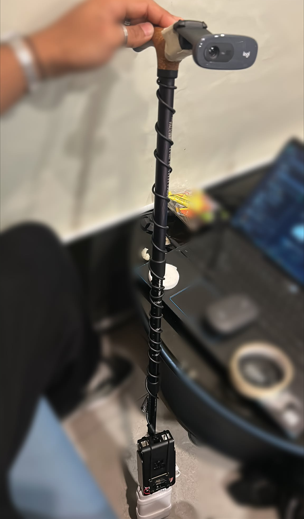
\includegraphics[height=8cm,keepaspectratio]{../photos/hardwarePhoto2.png}
\caption{Assembled prototype: Raspberry Pi 4, Arducam ToF camera (CSI), and USB webcam.}
\end{figure}

\subsection{Software Architecture}
The codebase is a modular Python package (\texttt{nav\_assistant}) organized by concern:

\begin{table}[H]
\centering
\begin{tabularx}{\textwidth}{l X}
\toprule
\textbf{Module} & \textbf{Responsibility} \\
\midrule
\texttt{sensors/} & Hardware abstraction for the webcam and ToF camera, with automatic V4L2 device detection by name \\
\texttt{mapping/} & Waypoint data model (SQLite + \texttt{.npy} ORB descriptors), distinguishing \texttt{location} vs.\ \texttt{landmark} kinds \\
\texttt{localization/} & ORB-based place/landmark recognition (classical CV) \\
\texttt{obstacle/} & ToF depth threshold detection \\
\texttt{perception/} & YOLOv8-nano obstacle classification (deep learning) \\
\texttt{speech/} & Vosk offline speech-to-text for destination input (deep learning) \\
\texttt{navigation/} & Reactive wall-following guided navigation \\
\texttt{audio/} & Text-to-speech (espeak-ng) and alert tones \\
\bottomrule
\end{tabularx}
\caption{Software module structure.}
\end{table}

\subsection{AI / Machine Learning Components}
\label{sec:ai}
The project guidelines require an explicit AI (ML/DL) component. Three recognition techniques are used deliberately, each chosen for where it performs best on constrained edge hardware:

\begin{enumerate}[leftmargin=1.4cm]
  \item \textbf{ORB feature matching} (classical computer vision, not learned) — used for visual place and landmark recognition. Chosen because it requires no training data beyond a short capture session, runs entirely on CPU, and is deterministic and debuggable.
  \item \textbf{YOLOv8-nano} (convolutional neural network, deep learning) — a pretrained, COCO-trained object detector (80 classes, $\sim$6MB) used to classify what triggered a ToF obstacle alert (e.g. ``chair'', ``person''), turning a generic alert into a specific one.
  \item \textbf{Vosk speech recognition} (deep neural network acoustic model) — used for fully offline voice destination input, with no cloud speech API involved.
\end{enumerate}

\subsubsection{Dataset Sources}
\label{sec:datasets}
Each technique has a fundamentally different relationship to training data, summarized in Table~\ref{tab:datasets}.

\begin{table}[H]
\centering
\begin{tabularx}{\textwidth}{l X}
\toprule
\textbf{Technique} & \textbf{Dataset source} \\
\midrule
ORB feature matching & \textbf{No external dataset.} Descriptors come entirely from the user's own environment, captured at runtime via the 2-minute training session (Table~\ref{tab:cv-vs-dl}; implemented in \texttt{mapping/recorder.py}). Nothing is pretrained; nothing is shared between deployments. \\
YOLOv8-nano & \textbf{Microsoft COCO} (Common Objects in Context) — a public benchmark dataset of $\sim$330{,}000 images covering 80 object categories and $\sim$1.5 million labeled object instances. We use the publicly released, COCO-pretrained weights (\texttt{yolov8n.pt}) as distributed by Ultralytics, with no project-specific fine-tuning. \\
Vosk speech recognizer & \texttt{vosk-model-small-en-us-0.15} (40MB), a publicly released English acoustic and language model distributed by Alphacephei, the Vosk maintainers, trained on public English speech corpora. We use the released model directly, with no project-specific fine-tuning or additional training data. \\
\bottomrule
\end{tabularx}
\caption{Dataset source for each AI/ML component used in the project.}
\label{tab:datasets}
\end{table}

\noindent Published accuracy benchmarks for the two pretrained models, as reported by their respective maintainers (not independently re-measured by us, since this would require either the original held-out test sets or hardware we no longer have access to):

\begin{itemize}[leftmargin=1.4cm]
  \item \textbf{YOLOv8-nano}: mAP\textsubscript{50-95} = 37.3 on the COCO \texttt{val2017} benchmark, 3.2M parameters (Ultralytics official model documentation).
  \item \textbf{Vosk small English model}: word error rate (WER) of 9.85\% on LibriSpeech \texttt{test-clean} and 10.38\% on TEDLIUM (Vosk official model page).
\end{itemize}

\subsubsection{Why YOLO Inference Is Gated, Not Continuous}
Running a CNN on every frame would be too slow for real-time use on a Raspberry Pi 4 CPU (no GPU). The architecture instead gates the deep learning inference behind the cheap ToF depth threshold: \texttt{ObstacleDetector} runs every cycle as before, and YOLOv8-nano only runs on the corresponding webcam frame \emph{after} an obstacle has already been flagged. This keeps the system real-time while still using a genuine deep learning model for recognition, illustrated in Listing~\ref{lst:yolo}.

\begin{lstlisting}[caption={Obstacle classification gated behind the cheap depth check (\texttt{perception/object\_detector.py}).}, label={lst:yolo}]
def classify(self, bgr_frame: np.ndarray) -> Optional[DetectionResult]:
    """Return the highest-confidence detection in the frame, or None."""
    if not self.is_available:
        return None

    results = self._model.predict(bgr_frame, verbose=False)[0]
    if results.boxes is None or len(results.boxes) == 0:
        return None

    best_idx = int(results.boxes.conf.argmax())
    confidence = float(results.boxes.conf[best_idx])
    if confidence < self._confidence_threshold:
        return None

    class_id = int(results.boxes.cls[best_idx])
    label = self._model.names[class_id]
    return DetectionResult(label=label, confidence=confidence)
\end{lstlisting}

\subsubsection{Why ORB Is Used for Landmarks, Not YOLO}
``Door'' is not a class in the COCO dataset that YOLOv8-nano is pretrained on, and fine-tuning a custom YOLO class would require collecting and labeling a training dataset — impractical within the project timeline. Trained ORB landmarks (Listing~\ref{lst:wall}) solve this with a two-minute capture session per landmark and no labeled dataset, at the cost of being less robust to lighting and viewpoint changes than a learned detector.

\subsection{Guided Navigation Decision Flow}
Figure~\ref{fig:navflow} illustrates the per-cycle decision sequence implemented by \texttt{GuidedNavigator.evaluate()}: arrival is always checked first (highest priority, ends the session), then a landmark announcement is composed if relevant, and finally the wall-following turn/straight decision is computed from the three ToF zones.

\begin{figure}[H]
\centering
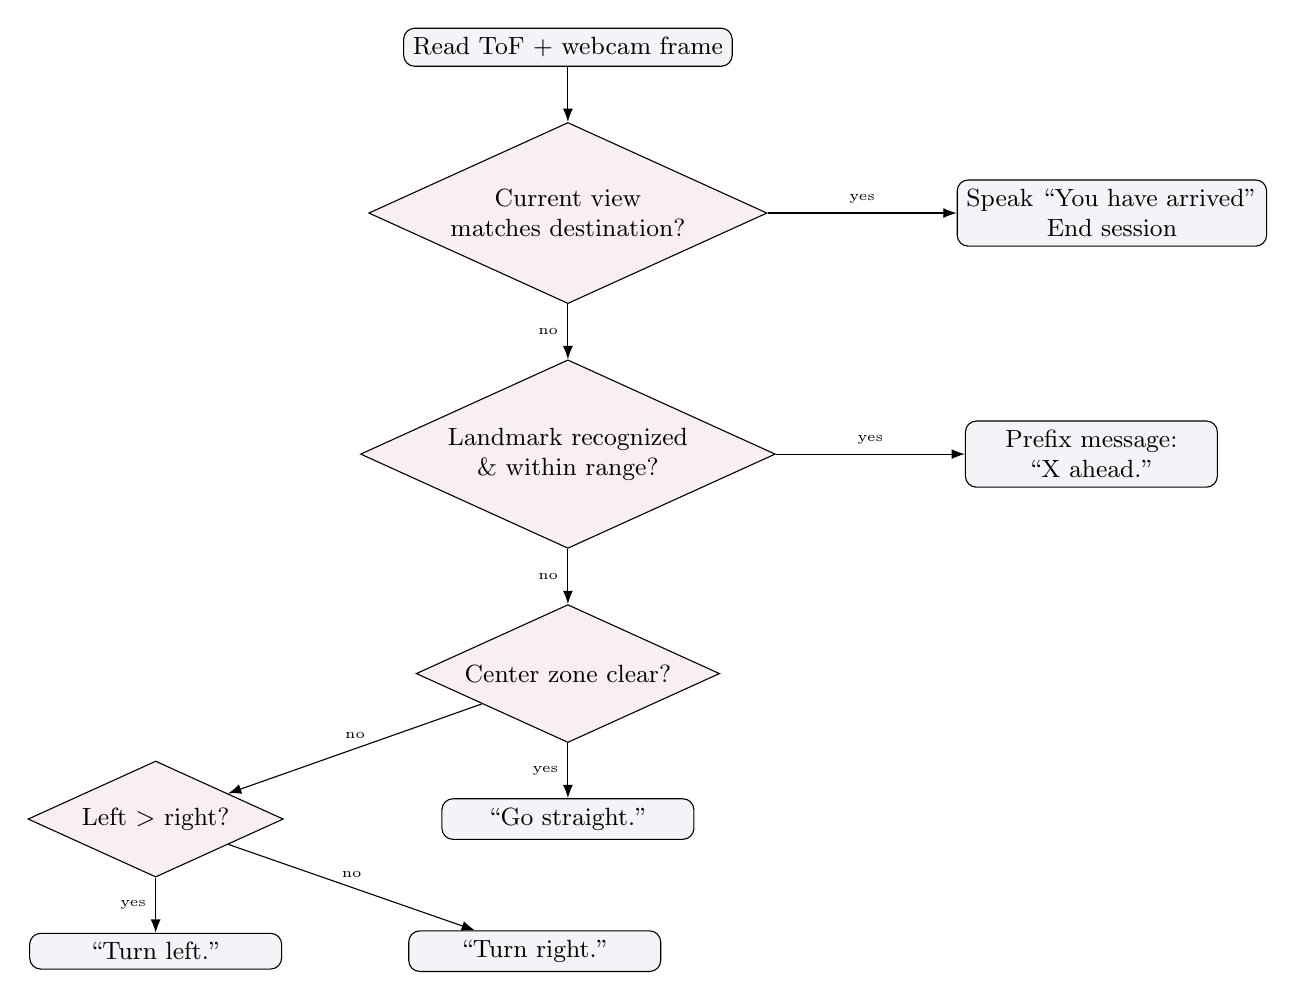
\begin{tikzpicture}[
  node distance=0.7cm and 0.6cm,
  decision/.style={diamond, draw, aspect=2.2, align=center, font=\small, fill=accent!8},
  action/.style={rectangle, draw, rounded corners, align=center, font=\small, fill=codebg, minimum width=3.2cm},
]
\node[action] (start) {Read ToF + webcam frame};
\node[decision, below=of start] (arrived) {Current view\\matches destination?};
\node[action, right=2.4cm of arrived] (sayarrived) {Speak ``You have arrived''\\End session};
\node[decision, below=of arrived] (landmark) {Landmark recognized\\\& within range?};
\node[action, right=2.4cm of landmark] (saylandmark) {Prefix message:\\``X ahead.''};
\node[decision, below=of landmark] (center) {Center zone clear?};
\node[action, below=of center] (straight) {``Go straight.''};
\node[decision, left=2.0cm of straight] (sides) {Left $>$ right?};
\node[action, below=of sides] (turnleft) {``Turn left.''};
\node[action, right=1.6cm of turnleft] (turnright) {``Turn right.''};

\draw[-Latex] (start) -- (arrived);
\draw[-Latex] (arrived) -- node[above,font=\tiny]{yes} (sayarrived);
\draw[-Latex] (arrived) -- node[left,font=\tiny]{no} (landmark);
\draw[-Latex] (landmark) -- node[above,font=\tiny]{yes} (saylandmark);
\draw[-Latex] (landmark) -- node[left,font=\tiny]{no} (center);
\draw[-Latex] (center) -- node[left,font=\tiny]{yes} (straight);
\draw[-Latex] (center) -- node[above,font=\tiny]{no} (sides);
\draw[-Latex] (sides) -- node[left,font=\tiny]{yes} (turnleft);
\draw[-Latex] (sides) -- node[above,font=\tiny]{no} (turnright);
\end{tikzpicture}
\caption{Decision flow for one guided-navigation cycle.}
\label{fig:navflow}
\end{figure}

\begin{lstlisting}[caption={Reactive wall-following decision logic (\texttt{navigation/guided\_navigator.py}).}, label={lst:wall}]
def _wall_following(self, left: float, center: float, right: float):
    if center <= 0 or center > self._clear_distance:
        return GuidanceResult(NavCommand.STRAIGHT, "Go straight.")

    if left <= 0 and right <= 0:
        return GuidanceResult(NavCommand.STOP, "Path blocked. Please stop.")

    if left > right:
        return GuidanceResult(NavCommand.TURN_LEFT, "Turn left.")
    elif right > left:
        return GuidanceResult(NavCommand.TURN_RIGHT, "Turn right.")
    else:
        return GuidanceResult(NavCommand.STOP, "Path blocked. Please stop.")
\end{lstlisting}

\subsection{Key Configuration Parameters}
All thresholds are externalized to a single YAML configuration file rather than hardcoded, allowing the system to be re-tuned for a new environment without code changes.

\begin{table}[H]
\centering
\begin{tabularx}{\textwidth}{l l X}
\toprule
\textbf{Parameter} & \textbf{Default} & \textbf{Purpose} \\
\midrule
\texttt{obstacle.alert\_threshold\_m} & 1.2 m & Distance below which an obstacle alert fires (awareness mode) \\
\texttt{navigation.clear\_distance\_m} & 1.0 m & Center-zone depth above which the path is ``clear'' (guided navigation) \\
\texttt{navigation.emergency\_threshold\_m} & 0.4 m & Tight safety override for something dangerously close \\
\texttt{navigation.landmark\_distance\_m} & 1.5 m & Maximum distance for a landmark to be announced \\
\texttt{localization.min\_good\_matches} & 15 & Minimum ORB matches to accept a recognition \\
\texttt{localization.confidence\_threshold} & 0.6 & Minimum confidence (0--1) to commit to a recognition \\
\texttt{perception.confidence\_threshold} & 0.5 & Minimum YOLO detection confidence to report \\
\bottomrule
\end{tabularx}
\caption{Selected tunable parameters from \texttt{config/default.yaml}.}
\label{tab:config}
\end{table}

% ===================================================================
\section{Results \& Contributions}
% ===================================================================

\subsection{Current Status}

\begin{table}[H]
\centering
\begin{tabularx}{\textwidth}{l l X}
\toprule
\textbf{Phase} & \textbf{Status} & \textbf{Outcome} \\
\midrule
Sensor integration & Complete & Webcam and ToF camera validated on real hardware with automatic device detection \\
Location training & Complete & Multiple locations trained, each with 1000\textendash5000 ORB descriptors \\
Awareness loop & Complete & Real-time obstacle alerts and location announcements running end-to-end \\
Guided navigation & Implemented & Voice input, wall-following, landmark announcement, arrival detection coded and unit-tested \\
DL obstacle classification & Implemented & YOLOv8-nano integrated, gated behind ToF threshold \\
\bottomrule
\end{tabularx}
\caption{Project status by phase.}
\end{table}

\subsection{Accuracy \& Robustness Validation}
\label{sec:accuracy}
The Raspberry Pi hardware used during development was not available at submission time, so end-to-end accuracy could not be re-measured on the deployed platform. Two complementary, honestly-scoped sources of evidence are used instead.

\subsubsection{Pretrained Model Benchmarks (YOLOv8-nano, Vosk)}
For the two deep learning components, we report the official published benchmarks from each model's maintainer (Section~\ref{sec:datasets}) rather than re-deriving new numbers without the original test sets: YOLOv8-nano reaches mAP\textsubscript{50-95} = 37.3 on COCO \texttt{val2017}; the Vosk small English model reaches a 9.85\% word error rate on LibriSpeech \texttt{test-clean}. Both are pretrained, unmodified, publicly verifiable figures.

\subsubsection{Controlled ORB Robustness Test (This Work)}
For the project's own classical-CV component, we ran a controlled desktop test: one reference photograph stands in for a ``trained location,'' and the exact production matching code (\texttt{place\_recognizer.py} — ORB with 500 features, BFMatcher, Lowe's ratio 0.75, \texttt{min\_good\_matches}=15, \texttt{confidence\_threshold}=0.6) is used to match synthetically perturbed versions of that photo against the original. This characterizes ORB's sensitivity to the same kinds of change a user introduces by viewing a location from a different angle, while moving, or under different lighting — directly relevant to the path-deviation discussion in Section~\ref{sec:deviation}. It is a single-image desktop validation, not a statistically representative field accuracy figure for the deployed system. The test script and raw results are included in the project repository at \texttt{docs/report/validation/} for reproducibility.

\begin{table}[H]
\centering
\begin{tabularx}{\textwidth}{l X X}
\toprule
\textbf{Perturbation} & \textbf{Result} & \textbf{Recognition threshold crossed} \\
\midrule
In-plane rotation (0\textdegree--90\textdegree) & Good matches stayed above 375/500 at every angle tested & Never failed — ORB's built-in rotation invariance held \\
Gaussian blur (simulating motion blur) & Good matches fell from 500 (none) to 144 (heavy blur, kernel 15) to 79 (kernel 21) & Failed (confidence $<$ 0.6) at kernel $\geq$ 15 \\
Brightness decrease (darker) & Good matches fell from 500 (unchanged) to 133 ($-$40) to 27 ($-$60) & Failed at $-$40 and below \\
Brightness increase (brighter) & Good matches remained $\geq$ 400 across all levels tested ($+$20 to $+$60) & Never failed \\
\bottomrule
\end{tabularx}
\caption{ORB recognition robustness under synthetic perturbations of a single reference image, using the exact production matching parameters.}
\label{tab:orb-robustness}
\end{table}

\noindent \textbf{Interpretation.} In-plane rotation alone is not a faithful proxy for the 3D viewpoint change a user introduces by approaching a location from a different angle (real viewpoint change also introduces perspective distortion, which this test does not capture) — so the true robustness to walking a different path is likely \emph{lower} than the rotation row suggests. The blur and darkening results, however, are directly informative: they indicate degraded lighting or fast head/cane movement is more likely to cause a missed recognition than camera angle alone, which directly explains the failure mode described in Section~\ref{sec:deviation}.

\subsection{Contributions}
\begin{itemize}[leftmargin=1.4cm]
  \item A working, fully offline assistive prototype combining depth sensing, computer vision, and two deep learning models on a single Raspberry Pi 4.
  \item A deliberate, documented architecture that pairs classical CV (ORB) and deep learning (YOLO, Vosk) by matching each technique to where it performs best, rather than defaulting to one approach.
  \item A robust hardware abstraction layer that automatically detects camera devices by name, solving a real instability (USB device indices changing across reboots) discovered during development.
  \item 27 automated unit tests covering the data model, sensor processing, navigation decision logic, and DL integration's graceful degradation.
\end{itemize}

\subsection{Engineering Challenges}
This section focuses on the four challenges that most shaped the project's architecture and process, rather than a full bug list (several smaller hardware integration fixes are documented in the project's change history).

\subsubsection{Challenge 1: Full SLAM Was Infeasible — Redesigning Around It}
The original project plan was full Visual SLAM (e.g. ORB-SLAM3): build a 3D map in real time and plan routes to arbitrary destinations. Partway into development it became clear this was not achievable with the available hardware and timeline — there is no IMU, no wheel odometry, and a single CPU-only Raspberry Pi 4, all of which SLAM implementations typically depend on for motion estimation between frames. Rather than attempting it anyway and shipping an unreliable map, we treated this as a scope decision, not a failure: the system was redesigned around two narrower but achievable modes — passive awareness and reactive wall-following guided navigation (Sections~\ref{sec:design}--\ref{sec:deviation}) — while keeping SLAM as an explicit, documented future-work item (Section~\ref{sec:future}) rather than silently dropping it.

\subsubsection{Challenge 2: Training Data Evolved Through Three Iterations}
Visual place recognition's reliability turned out to depend heavily on how training data was collected, which we only discovered by testing the simplest approach first:
\begin{enumerate}[leftmargin=1.4cm]
  \item \textit{Single frame.} The first implementation captured one webcam frame per location. Recognition was unreliable — a single viewpoint does not capture enough visual diversity for ORB to match later, naturally varying views.
  \item \textit{Short burst.} Capturing 5 frames in quick succession improved things slightly, but frames taken within roughly a second of each other are still nearly the same viewpoint, so diversity barely improved.
  \item \textit{Continuous two-minute capture (final).} The training tool now samples one frame every 3 seconds for 2 minutes while the user walks around the space, yielding $\sim$40 frames and up to 5{,}000 descriptors per location (randomly subsampled if more are collected, to bound matching cost). This is also the data source documented in Table~\ref{tab:datasets} for ORB's ``no external dataset'' design.
\end{enumerate}
This is a direct, practical illustration of why dataset \emph{construction methodology} matters as much as dataset \emph{size} for a classical CV technique with no learned generalization.

\subsubsection{Challenge 3: A Thread-Safety Bug That Only Appeared on a Different Platform}
While preparing this submission without access to the Raspberry Pi, we built a desktop demo tool (running on Windows) and discovered a real bug invisible on the original target platform: the \texttt{pyttsx3} text-to-speech fallback shares one engine instance between a background ``speak'' thread and the main thread's ``alert'' call. On Windows, \texttt{pyttsx3}'s SAPI5 driver is COM-based and apartment-threaded, meaning a single engine instance may only safely be called from the thread that created it — calling it from a second thread silently hangs with no exception. The fix creates a fresh, short-lived engine inside every call, scoped entirely to whichever thread is using it. This had no effect on the Raspberry Pi, which uses the \texttt{espeak-ng} subprocess backend instead (each call is an independent process, inherently thread-safe) — but would have caused a hard-to-diagnose hang for any future Windows or macOS deployment.

\subsubsection{Challenge 4: Gating Deep Learning Inference Behind a Cheap Check}
Running YOLOv8-nano on every frame would be too slow for real-time use on a CPU-only Raspberry Pi 4. The solution (Section~\ref{sec:ai}) runs the cheap ToF depth threshold every cycle as before, and only invokes the CNN on the webcam frame after an obstacle has already been flagged — paying the deep learning inference cost only when it is actually useful.

% ===================================================================
\section{Future Work}
\label{sec:future}
% ===================================================================

The features below were part of the original project vision and were consciously deferred to keep the current scope achievable within the term:

\begin{itemize}[leftmargin=1.4cm]
  \item \textbf{Visual SLAM} — building a 3D map of the environment in real time (e.g. ORB-SLAM3) instead of reactive wall-following, enabling navigation to destinations not directly visible.
  \item \textbf{Graph-based route planning} — the data model already stores directed edges between locations (\texttt{WaypointEdge}); a Dijkstra-based planner could route across multiple reactive legs.
  \item \textbf{IMU integration} — dead-reckoning between locations would allow distance and orientation tracking independent of visual recognition.
  \item \textbf{Fine-tuned object detection} — training a custom YOLO model on assistive-technology-relevant classes (doors, stairs, curbs) instead of relying on ORB landmarks and generic COCO classes.
  \item \textbf{Multi-environment support} — automatic environment selection when the device is carried between different trained spaces.
\end{itemize}

% ===================================================================
\section{Conclusion}
% ===================================================================

This project demonstrates that a meaningful assistive navigation system can be built entirely offline on commodity Raspberry Pi hardware by combining classical computer vision and deep learning where each is most effective. Rather than attempting full SLAM-based navigation with insufficient sensors and time, the team redesigned the scope around two achievable, genuinely useful modes — environmental awareness and reactive guided navigation — while explicitly preserving the original ambitions as a documented roadmap. The resulting system detects and classifies obstacles, recognizes trained locations, accepts voice commands, and gives turn-by-turn audio guidance, all without an internet connection.

\end{document}
